% informativeness.tex

\begin{figure}[t]
  \centering
    \begin{subfigure}[b]{0.40\textwidth}
        \centering
        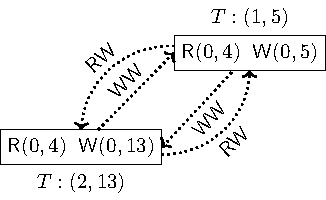
\includegraphics[width = \textwidth]{figs/galera-original}
        \caption{Original output}
    \end{subfigure}\hspace{3ex} \pause
    \begin{subfigure}[b]{0.40\textwidth}
        \centering
        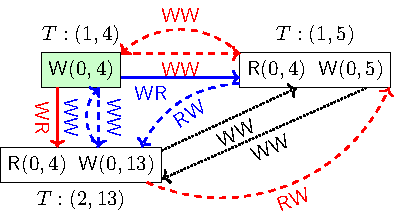
\includegraphics[width = \textwidth]{figs/galera-recovery-1}
        \caption{Missing  participants}
    \end{subfigure}\hspace{3ex} \pause
    \begin{subfigure}[b]{0.40\textwidth}
        \centering
        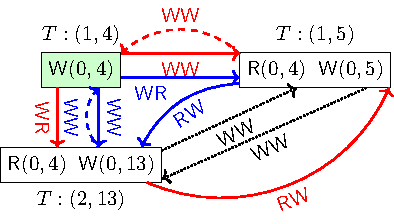
\includegraphics[width = \textwidth]{figs/galera-recovery-2}
        \caption{Recovered scenario}
    \end{subfigure}\hspace{3ex} \pause
    \begin{subfigure}[b]{0.40\textwidth}
        \centering
        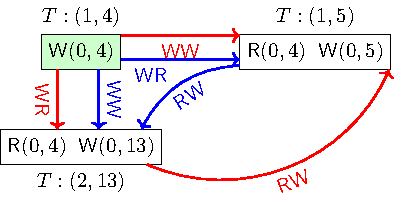
\includegraphics[width = \textwidth]{figs/galera-delete}
        \caption{Finalized scenario}
    \end{subfigure}
%     \caption{\label{ce:galera}  Lost update: the SI violation  found in MariaDB-Galera.
%     The original output dependencies  are represented by dotted black arrows.
%     The recovered dependencies are colored in red/blue with dashed and solid arrows  representing uncertain  and certain dependencies,  respectively.  The  missing transaction is colored in green.
% We omit  key 0, associated with all dependencies.    }
\end{figure}